\documentclass[conference]{IEEEtran}
\usepackage{enumerate}
\usepackage{hyperref}
\usepackage{todonotes}
\usepackage[framemethod=TikZ]{mdframed}
\usepackage{graphicx}
\newmdenv [ %
 skipabove=\topsep,
 skipbelow=\topsep,
 roundcorner = 5pt,
 leftmargin = 2,
 rightmargin = 2,
 % backgroundcolor = oldlace,
 innertopmargin = 3,
 splittopskip = 3]{mq}
\ifCLASSINFOpdf
 \else
 \fi
\begin{document}

\title{Utilizando a Fase de Empatia do Design Thinking como Facilitadora na Elicitação dos Requisitos de Privacidade
}
\author{\IEEEauthorblockN{Edna Dias Canedo}
\IEEEauthorblockA{Department of Computer Science \\ University of Bras\'{i}lia (UnB)\\
P.O. Box 4466, Bras\'{i}lia--DF, Brazil \\
Email: ednacanedo@unb.br}
\and
\IEEEauthorblockN{Angelica Toffano Seidel Calazans}
\IEEEauthorblockA{University center -- UniCEUB\\
Bras\'{i}lia--DF, Brazil \\
Email: angelica.toffano@gmail.com}
\and

\IEEEauthorblockN{Anderson Jefferson Cerqueira}
\IEEEauthorblockA{Department of Computer Science \\ University of Bras\'{i}lia (UnB)\\
P.O. Box 4466, Bras\'{i}lia--DF, Brazil \\
Email: andersonjcdf@gmail.com}
}
\maketitle

\begin{abstract}
%Este artigo apresenta uma contextualização do uso da Phase de Empatia no processo de elicitação de requisitos de privacidade. Nós realizamos uma revisão de literatura para identificar o uso do da Phase de Empatia do Design Thinking na elicitação de requisitos de privacidade. Além disso, nós realizamos um survey com 63 profissionais da indústria para entender como é realizado a elicitação desses requisitos e se estes profissionais utilizam a Phase de Empatia. Nós identificamos que 73.9\% dos desenvolvedores utilizam a fase de empatia para elicitar os requisitos de software. Por fim, nós propomos um modelo de empatia que poderá ser utilizado pelos desenvolvedores de software no processo de elicitação dos requisitos de privacidade.%

This article presents a contextualization of the use of the Empathy Phase in the process of eliciting privacy requirements. We conducted a literature review to identify the use of the Design Thinking Empathy Phase in eliciting privacy requirements. In addition, we conducted a survey with 63 industry professionals to understand how these requirements are elicited and whether these professionals use the Empathy Phase. We found that 73.9 \% of developers use the empathy phase to elicit software requirements. Finally, we propose an empathy model that can be used by software developers in the process of eliciting privacy requirements.

\end{abstract}
\IEEEpeerreviewmaketitle

\section{Introduction}

Com o surgimento de novas tecnologias e legislações, a proteção dos dados dos usuários precisa ser considerada durante todo o processo de desenvolvimento de software. Para implementar uma funcionalidade de um software que irá fazer uso de dados pessoais, é necessário que seja considerado os requisitos de privacidade durante a fase de elicitação de requisitos \cite{DBLP:conf/wer/NettoPS19}. A General Data Protection Regulation (GDPR) \cite{Eu2019} e a Brazilian General Data Protection Law (LGPD) \cite{leiLGPD} são leis que definem a proteção dos dados pessoais, e nas quais, fica evidente que os usuários têm o direito de receber as informações de forma clara e precisa sobre como seus dados serão tratados \cite{DBLP:conf/re/Ayala-RiveraP18}. Assim, garantir a privacidade dos dados dos usuários se tornou uma das principais preocupações no desenvolvimento de software, seja para satisfazer as necessidades dos usuários ou para cumprir as leis de privacidade em vigor \cite{DBLP:conf/sbes/PeixotoS18}, \cite{DBLP:conf/wer/NettoPS19}, \cite{DBLP:conf/amcis/HuthM19}, \cite{DBLP:conf/IEEEares/HorakSH19}.

Os dados dos usuários devem ser protegidos antes do seu armazenamento e quando os sistemas de software apresentarem informações oriundas da análise dos dados dos usuários que foram coletados, o software deve utilizar proteções que não permitam a restauração de informações (identificação do proprietário do dado), ou seja, o armazenamento não deve permitir a restauração dos dados após a aplicação de uma solução de privacidade \cite{Eu2019},\cite{leiLGPD}. Existem diversas soluções propostas para a proteção da privacidade dos dados do usuário, dentre essas soluções, as que modificam atributos; e as que não modificam os atributos \cite{DBLP:journals/iotj/Vergara-Laurens17}.

As soluções que modificam os atributos compreendem técnicas que aplicam algoritmos para agrupar, ofuscar, anonimizar, minimizar, dentre outras, alterando a estrutura dos dados para impedir a identificação de um indivíduo no grupo. As soluções que não modificam os atributos são técnicas que aplicam algoritmos de proteção sem alteração das informações, tais como encriptação, criptografia homomórfica, etc. \cite{DBLP:journals/iotj/Vergara-Laurens17}.

Desenvolver sistemas de software que garantem a proteção dos dados pessoais é um desafio para os desenvolvedores de software, tornando-se mais complexo quando envolvem sistemas distribuídos, que podem possuir diversas formas de coleta de dados dos usuários, como ocorre na maioria das aplicações comerciais e ou governamentais. Além disso, a proteção dos dados é essencial para obter a confiança e a participação dos usuários no processo de coleta de dados. Para atender a essa necessidade de proteção de dados, é preciso adotar e utilizar novas técnicas e ferramentas para elicitar os requisitos e analisar e disponibilizar os dados pessoais. Uma maneira de facilitar o processo de elicitação de requisitos de privacidade pode ser o uso do mapa de empatia \cite{DBLP:conf/sbes/FerreiraCB15} e do Design Thinking \cite{DBLP:books/lib/brown2009change}, \cite{DBLP:conf/hci/CanedoC18}. 

Assim, o objetivo desta pesquisa é identificar como a fase de Empatia do Design Thinking pode ser utilizada como ferramenta facilitadora na elicitação dos requisitos de privacidade. Altogether, in this work we answer questions related to (a) a utilização da fase de empatia do Design Thinking na elicitação de requisitos de privacidade and (b) as ferramentas que podem ser utilizadas na fase de empatia para elicitar os requisitos de privacidade de uma maneira mais clara e eficaz. Accordingly, we present the following contributions:

\begin{itemize}
    \item \textcolor{red}{No final colocar aqui os principais achados do artigo}.
\end{itemize}

Este artigo está organizado como segue. Na Seção \ref{back} é apresentado uma contextualização sobre os principais conceitos relacionados a essa pesquisa e os trabalhos correlatos. Na Seção \ref{method} é apresentada a metodologia utilizada para conduzir este trabalho. Na Seção \ref{empathy} é apresentado um survey para compreender a percepção dos desenvolvedores de software do uso da Empatia e do Design Thinking na elicitação dos requisitos de privacidade. As ameaças para a validação dessa pesquisa são apresentadas na Seção \ref{thread}. Por fim, as conclusões e trabalhos futuros são apresentados na Seção \ref{conclusion}.

\section{Background}
\label{back}
\subsection{Design Thinking}

O Design Thinking considera que a tarefa mais importante ao iniciar um projeto de desenvolvimento de software é entender as necessidades dos usuários, investigando quais são as suas necessidades e qual impacto o software causaria com o seu uso. Todos os participantes do processo de desenvolvimento procuram entender o universo do usuário com o objetivo de obter as informações necessárias para a elicitação dos requisitos e as percepções dos usuários em relação a elas \cite{DBLP:books/lib/brown2009change}. Assim, a ideia principal do Design Thinking é como os designers progridem com o processo de desenvolvimento, com ideias criativas para as soluções propostas, no intuito de descobrir e oferecer novas oportunidades \cite{DBLP:conf/hci/AdikariMC13}. O Design Thinking dissemina a inovação centrada no usuário, de modo que exista colaboração, interação e abordagens práticas para encontrar as ideias mais apropriadas e, consequentemente, soluções coerentes para os problemas dos usuários \cite{DBLP:books/lib/brown2009change}. 

\subsubsection{Fases do Design Thinking}

No contexto de Engenharia de Software, existem diversos modelos de Design Thinking com diferentes stages. Os modelos propostos por Sandino et al. \cite{DBLP:conf/hci/SandinoMV13}, Hiremath e Sathiyam \cite{DBLP:conf/interact/HiremathS13} and Coutinho et al. \cite{DBLP:conf/eatis/CoutinhoGJ16} apresentam sete fases. De Paula e Araújo \cite{DBLP:conf/hci/PaulaA16} propuseram um modelo de Design Thinking de seis fases associado ao processo de desenvolvimento ágil e Lean Startup. 
Newman et al. \cite{DBLP:conf/icse/NewmanFSFFW15} apresentaram o DrivingBoard, um modelo de Design Thinking de 6 fases que utiliza Design Participativo e Desenvolvimento Ágil. Ximenes et al.  \cite{DBLP:conf/hci/XimenesAA15} combinaram Design Thinking, Lean Startup e Desenvolvimento Ágil. O Design Thinking utilizado pelos autores foi o modelo proposto pela Stanford University’s D-School e neste trabalho nós iremos utilizar esse modelo, o qual possui 5 fases, dentre elas a fase de empatia \cite{DBLP:conf/hci/XimenesAA15}, conforme apresentado na Figura \ref{fig:my_label}: 

\begin{enumerate}

\item Empatia: Esta fase é primordial para obter uma visão geral do usuário. É uma fase de conhecimento sobre as  necessidades e desejos dos usuários. A empatia é usada para ouvir, ver e sentir. É perceber o usuário, colocar-se no lugar dele e enxergar o quê, como e quando uma ação é possível em busca de uma solução para o problema.

\item Definição: Esta etapa talvez seja uma das mais desafiadoras, uma vez que envolve a interpretação de todos os fatos adquiridos no processo de empatia. Para que uma definição do problema seja atingida, é preciso processar tudo o que foi dito e visto na etapa de Empatia, o que pode ser uma atividade bastante trabalhosa e demorada.

\item Ideação: É uma fase muito abrangente, na qual as ideias e os conceitos são gerados com o objetivo de gerar inovações sobre os problemas identificados na etapa de Empatia e Definição. 

\item Prototipação: Nesta fase se faz necessário construir protótipos para as ideias aprovadas. A principal função desses protótipos é permitir um teste rápido de uma ideia tangível, mesmo que seja de baixa fidelidade. Os protótipos permitem um feedback rápido dos usuários e são rápidos de fabricar, além de baratos.
    
\item Teste: Esta é a última fase, sendo a hora de apresentar os protótipos criados ao usuário e buscar feedback. Essa etapa serve para refinar ideias e soluções. os protótipos são avaliados com a prospectiva dos usuários finais para investigar se as ideias e os pressupostos manifestados nestes protótipos são consideradas soluções adequadas. Cada rodada de teste também é empática, pois as equipes aprendem muito observando como os usuários interagem com o produto. A diferença é que o teste faz com que a equipe de desenvolvimento ofereça necessariamente uma versão do produto (seja em papel, código ou qualquer outro meio aplicável) para o usuário interagir. Os testes reduzem os confrontos dentro da equipe. Isso deixa claro o que funciona melhor para o usuário. Os testes para um projeto de software criativo são muito parecidos com a engenharia de requisitos na metodologia ágil, ou seja, o usuário escolhe o que prefere. As equipes devem ser treinadas para entender quando estão fazendo hipóteses e assumindo coisas que deveriam ser testadas. 

\end{enumerate}

\begin{figure}
    \centering
    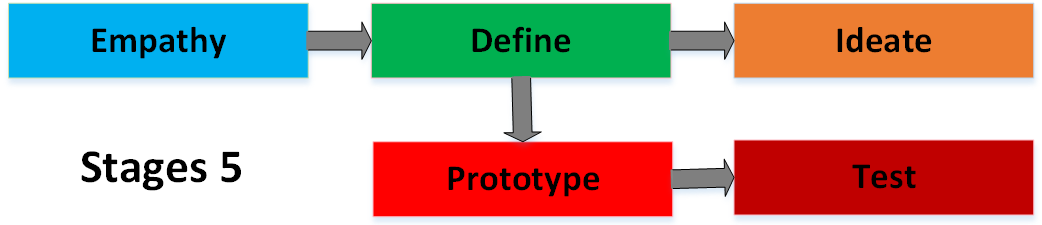
\includegraphics[width=3.2in]{Figures/5Stages.png}
    \caption{Stanford’s d.school Design Thinking and its Stages \cite{DBLP:conf/hci/XimenesAA15},\cite{ DBLP:conf/icse/CarrollR16}}
    \label{fig:my_label}
\end{figure}

Algumas ferramentas de apoio ao Design Thinking na fase de elicitação de requisitos são: \href{http://www.smaply.com}{Smaply}: ferramenta de persona e outros métodos tais como stakeholder map e customer journey maps; \href{http://www.stakeholder-management.com/}{Stakeholder Circle}: ferramenta de stakeholder maps; \href{http://www.touchpointdashboard.com}{Touchpoint  Dashcboard}: ferramenta de customer journey maps; \href{http://www.creately.com}{Creately}: ferramenta de service blueprint; \href{http://www.strategyzer.com}{Strategyzer}: ferramenta de business model innovation; \href{http://
www.axure.com/}{Axure RP}: ferramenta de prototipação rápida.

\subsection{Requisitos de Privacidade}
\cite{DBLP:conf/wer/2019}



\subsection{Trabalhos Correlatos}

\subsubsection{Mapa da Empatia}

O Mapa da Empatia (EM) é uma técnica que auxilia no design de modelos de negócios de acordo com às perspectivas dos usuários. Desenvolve um
melhor entendimento do ambiente, comportamento, aspirações e preocupações de um usuário \cite{DBLP:conf/hci/FerreiraBC16}.

\todo[inline]{Aqui descrever os trabalhos que utilizam a empatia na elicitação de requisitos}

\section{Study Settings}
\label{method}

In this section we describe the settings of our study. We first state the goal of our investigation, and then we present details about the research questions we address and the procedures we take to conduct the study and collect issues from privacy requirements elicitation.

In this section we describe the settings of our study. We first state the goal of our investigation, and then we present details about the research questions we address and the procedures we take to conduct the study and collect issues from privacy requirements elicitation.

\subsection{Research Goal}

The main goal of this research is identificar na literatura e na indústria como a fase de Empatia do Design Thinking pode ser utilizada como ferramenta facilitadora na elicitação dos requisitos de privacidade. Neste trabalho, o nosso foco é em projetos de desenvolvimento de software. 

\subsection{Research Questions}
\label{rq}  

We conduct a multi-method study to investigate the following research questions:

\begin{enumerate}[RQ.1:]
    \item Como a fase de Empatia do Design Thinking pode motivar o desenvolvedor de software a identificar e tratar de forma eficaz os requisitos de privacidade?
    \item Quais as ferramentas relacionadas à fase de Empatia podem ser utilizadas para facilitar a elicitação de requisitos de privacidade? 
    \item A Empatia está relacionada a uma habilidade do desenvolvedor de software ou a uma orientação organizacional (processo padronizado/definido pela organização)?

\end{enumerate}

Para responder a RQ.1 e RQ.3 nós realizamos um grupo focal com os desenvolvedores de software da polícia militar do distrito federal PMDF. Nós exploramos questões relacionadas a .......

Para responder a RQ.2 nós realizamos uma revisão de literatura para identificar as ferramentas que são utilizadas na fase de Empatia na elicitação de requisitos e quais dessas ferramentas podem facilitar a elicitação de requisitos de privacidade.

\subsection{Research Methods}

\todo[inline]{aqui descreveremos rapidamente como foi configurado o grupo focal}

\section{STUDY RESULTS}
\label{empathy}


A principal diferença da proposta do nosso trabalho para o modelo PATHY é que o nosso modelo proposto será validado com desenvolvedores de software.

\subsection{Empathy and Privacy Requirements}

\begin{mq}
\emph{"Por meio da empatia é fácil entender o ponto de vista do cidadão/usuário do sistema e suas reais necessidades e limitações."}
\end{mq}

\begin{mq}
\emph{"Como o desenvolvedor é também um facilitador, a fase de empatia é a que na minha experiência, mais elucida e anima o desenvolvedor a querer resolver os problemas apontados pelos usuários com que ele se relacionou. Vivenciar a realidade do usuário em muito dá propósito ao trabalho do desenvolvedor, além de permitir insumos para que ele pense em melhores soluções na parte de ideação."}
\end{mq}


\todo[inline]{responder a questão de pesquisa : RQ.2 e sempre referenciar as afirmações}

\subsection{Focal Group}

\todo[inline]{aqui descreveremos os resultados com o grupo focal}

%
%\begin{figure*}[!t]
%\centering
%\subfloat[Case I]{\includegraphics[width=2.5in]{box}%
%\label{fig_first_case}}
%\hfil
%\subfloat[Case II]{\includegraphics[width=2.5in]{box}%
%\label{fig_second_case}}
%\caption{Simulation results for the network.}
%\label{fig_sim}
%\end{figure*}
%

%\begin{table}[!t]
%% increase table row spacing, adjust to taste
%\renewcommand{\arraystretch}{1.3}
% if using array.sty, it might be a good idea to tweak the value of
% \extrarowheight as needed to properly center the text within the cells
%\caption{An Example of a Table}
%\label{table_example}
%\centering
%% Some packages, such as MDW tools, offer better commands for making tables
%% than the plain LaTeX2e tabular which is used here.
%\begin{tabular}{|c||c|}
%\hline
%One & Two\\
%\hline
%Three & Four\\
%\hline
%\end{tabular}
%\end{table}


\section{Threats to Validity}
\label{thread}

\todo[inline]{Aqui descrever as ameaças para validação da pesquisa -- ver modelos outros artigos, falar sobre as ameaças a condução da revisão de literatura, ao grupo focal e etc.}


\section{Conclusion}
\label{conclusion}

\section*{Acknowledgment}

\bibliographystyle{IEEEtran}
\bibliography{paper}

\end{document}


